% cheng to review
\subsection{Distributed Extent Management System}
\label{sec:cases:azurestore}

We used \psharp to test the \emph{distributed extent management} component of the Windows Azure vNext distributed storage system. This component is responsible for managing the partitioned extent metadata and works as follows.

There are multiple \emph{extent managers} (EMgrs) that are in charge of managing a subset of the extents. Each EMgr communicates asynchronously (via remote procedure calls) with a number of \emph{extent nodes} (ENs) that store the extents. Each EN sends: (i) a \emph{heartbeat} every 5 seconds, to notify the EMgr that it is still available; and (ii) a \emph{sync report} every 5 minutes, to synchronize its extent with the rest of the nodes. The EMgr contains two data structures: an \emph{extent center} (ECtr), which is updated every time an EN syncs; and an EN map, which is updated every time it receives a heartbeat from an EN. The EN map runs an EN expiration loop that is responsible for removing ENs that have expired from the EN map and also delete them from the ECtr. Finally, the EMgr runs an extent repair loop, which examines all contents of all extents in the ECtr and schedules repairs of extents if they are out-of-date (via a repair request).

\subsection{Live Azure Table Migration}

We also used \psharp to test the MigratingTable library, which is capable of transparently migrating a data set between tables in the Windows Azure storage service while an application is accessing the data set.  MigratingTable provides a ``virtual table'' with an API similar to that of an ordinary Azure table, backed by a pair of ``old'' and ``new''  tables.  It moves all data from the old table to the new table in the background.  Meanwhile, each read or write issued to the virtual table is translated to a sequence of reads and writes on the backend tables according to a protocol we designed, which guarantees linearizability of operations on the virtual table across multiple application processes assuming that the backend tables respect their own linearizability guarantees.

\begin{figure}[t]
\centering
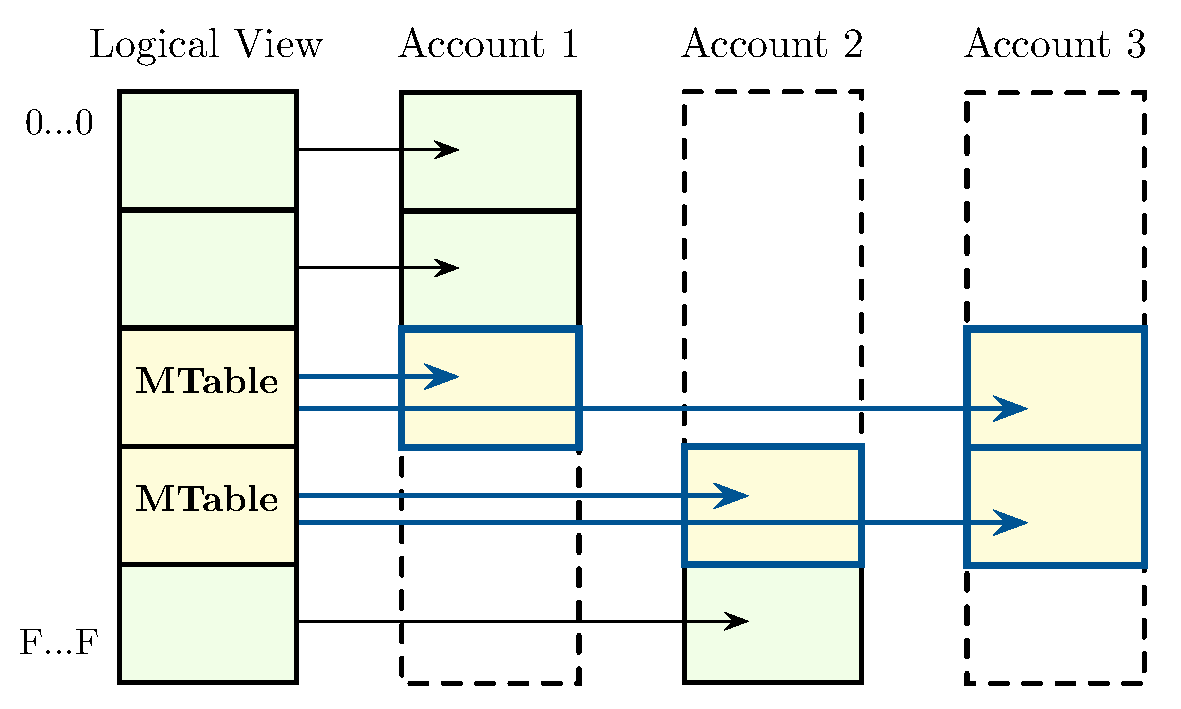
\includegraphics[width=\linewidth]{img/livemigration}
\caption{Draft.}
\label{fig:livemigration}
\end{figure}

% N.B. Artifact Services is mentioned at http://research.microsoft.com/en-us/people/schulte/.  Hopefully it's OK to reveal that it was the system in this case study. ~ Matt 2015-08-17
The initial motivation for MigratingTable was to solve a scaling problem for Artifact Services, an internal Microsoft system with a data set that is sharded across tables in different Azure storage accounts because it exceeds the limit on traffic supported by a single Azure storage account.  As the traffic continues to grow over time, we will need to reshard the data set across a greater number of Azure storage accounts without interrupting service.  During such a resharding, our sharding manager will identify each key range that should migrate to a different table, and we will use a separate MigratingTable instance for each such key range to actually perform the migration.  MigratingTable may also be useful to migrate data to a table with different values of configuration parameters that Azure does not support changing on an existing table, such as geographic location.

Since we were designing a new concurrent protocol that we expected to become increasingly complex over time as we add optimizations, we planned from the beginning to maintain a \psharp test harness along with the protocol to maintain confidence in its correctness.

\subsubsection{Modeling approach}
% TBD where this ends up in the paper ~ Matt 2015-08-17

MigratingTable implements an interface called IChainTable2, which provides the core read and write functionality of the real Azure table API with one exception: it provides a weaker consistency property for multi-page reads, since the original property would have been difficult to achieve for no benefit to applications we could foresee.  MigratingTable requires that its backend tables also implement IChainTable2, and we wrote a simple adapter to expose physical Azure tables as IChainTable2.  Our goal was then to verify that when multiple application processes issue ``input'' read and write calls to their own MigratingTable instances with the same backend tables, the behavior complies with the specification of IChainTable2 for the combined input history.

% N.B. SpecTable = InMemoryTableWithHistory in the current codebase. ~ Matt 2015-08-17
Since the specification is deterministic under sequential calls except for the results of multi-page reads, we decided the easiest way to formulate it for automated testing was to write an in-memory reference implementation called SpecTable.  Given a multi-page read, SpecTable can actually produce a list of all valid results.  Our correctness property is then:
\begin{quote}
For every execution trace of a collection of MigratingTables backed by the same pair of SpecTables (which nondeterministically choose one of the valid results for each multi-page read), there exists a linearization of the combined input history such that the output in the original trace matches the output of a ``reference'' SpecTable on the linearized input.
\end{quote}
%
\def\term#1{\emph{#1}}
We instrumented MigratingTable to report the \term{linearization point} of each input call, which in our case is always one of the corresponding \term{backend calls} to the backend tables (often the last).  Specifically, after each backend call completes, MigratingTable reports whether it was the linearization point, which may depend on the result of the call.  This makes it possible to verify the correctness property as the system executes.  We have a \psharp \term{tables machine} containing all three SpecTables and a collection of \term{service machines} each containing a MigratingTable.  Each service machine issues a random sequence of input calls to its MigratingTable, which sends backend calls to the tables machine.  When MigratingTable reports the linearization point of an input call, the service machine sends that input call to the reference table.  When an input call completes, the service machine checks that the results from the MigratingTable and the reference table agree.  \psharp controls the interleaving of the backend calls.  To ensure that the reference table is never observed to be out of sync with the backend tables, after the tables machine processes a backend call, it enters a state that defers further backend calls until MigratingTable has reported whether the backend call was a linearization point and (if so) the call to the reference table has been made.  We use the \psharp nondeterminism API to generate the input calls, so in principle an exhaustive \psharp behavior exploration strategy such as DFS could be used to exhaustively test MigratingTable up to some bound.

% Draft
We wanted to implement the core MigratingTable algorithms in \csharp ``async'' code, like most of Artifact Services.  Async code is readable like traditional procedural code but is translated by the compiler to an event-driven state machine using the Task Parallel Library, gaining most of the performance benefits of that style.  By default, all event processing occurs on the .NET thread pool.

We had to arrange for the continuations to execute within the context of a single \psharp machine, which we did by installing a custom SynchronizationContext.  Then we implemented async RPC between machines in terms of message passing, using RealProxy to avoid most of the marshaling boilerplate.
